\documentclass{article}

\usepackage{hyperref}
\usepackage{algorithm}
\usepackage{amsfonts}
\usepackage{amsmath}
\newtheorem{definition}{Definition}
\usepackage{algpseudocode}
\usepackage{graphicx}
\usepackage{enumitem}
\usepackage{pgfplots}
\pgfplotsset{width=6cm,compat=1.9}

\algrenewcommand\algorithmicrequire{\textbf{Input:}}
\algrenewcommand\algorithmicensure{\textbf{Output:}}
\usepackage{xcolor}

\title{\texttt{dpsa4fl}: Differential Privacy for Federated Machine Learning}
\author{Olivia Roehrig  \\
	Your Company / University  \\
	\and
	Maxim Urschumzew \\
	\textit{Determi} \\
	}

\date{\today}
% Hint: \title{what ever}, \author{who care} and \date{when ever} could stand 
% before or after the \begin{document} command 
% BUT the \maketitle command MUST come AFTER the \begin{document} command! 
\begin{document}

\maketitle


\begin{abstract}
Short introduction to subject of the paper \ldots 
\end{abstract}

\section{Introduction}
Data privacy is one of the factors motivating federated learning. A machine learning model can be trained locally on computers owned by data owners (clients), who exchange only intermediate training results (gradients), instead of the data itself, with a central server that aggregates them into a shared model~\cite{McMahan2016CommunicationEfficientLO}. While this relieves the need to collect possibly sensitive data in a central location to perform the training process, the shared model and the gradients themselves contain enough information to enable reconstruction of private information~\cite{7958568}\cite{Boenisch2021WhenTC}.

A solution to this problem is using a modified training algorithm that provides \emph{differential privacy} for the model~\cite{Abadi_2016}. The technique adds a small amount of noise to the result of each training step, calibrated in a way that makes high certainty statements about the presence of an individual point in the training dataset unlikely to be inferrable from the model.

In this document, we present an architecture that allows using federated gradient descent while providing differential privacy for the training result as well as all intermediate gradients.

Adding noise locally will require a large amount of noise and hence large utility loss to achieve privacy, so our protocol adds noise after aggregating intermediate results (\emph{global} differential privacy). To avoid revealing the non-noised aggregate to even the party adding the noise, we use the Prio protocol for \emph{secure aggregation}~\cite{prio}.

\paragraph{Prio.} The protocol has been designed by Corrigan-Gibbs and Boneh in~\cite{prio} as a
way to securely aggregate client data with two aggregation servers. As long as
one server remains honest, the data remains private. The outstanding feature of
prio is that the validity of the submitted data can be verified by the
aggregators without them having access to the data itself, by using a form of
zero-knowledge proofs. Such proofs are verified using arithmetic circuits, and
while prio provides a framework for implementing them, they have to be designed
for each specific use-case individually.

The original prio protocol has since been improved, and, under the name of Prio3, integrated into the
more general framework of \textit{verifiable distributed aggregation
  functions}~\cite{vdaf} (VDAFs). It is currently being implemented in the rust library
\texttt{libprio-rs}~\cite{libprio-rs}, in tandem with ongoing specification effort~\cite{vdaf-draft}.
VDAFs are meant to be executed using the \textit{distributed aggregation
  protocol}, currently being implemented in \texttt{janus}~\cite{janus}, with
specification ongoing in~\cite{dap-draft}.

For our federated learning system we use the implementation of Prio3
as implemented in \texttt{libprio-rs} and \texttt{janus}. Nevertheless, for our
explanations in the present paper
we mostly refer to the more compact presentation of the original protocol in~\cite{prio}.

\paragraph{Contributions.}
Our goal is to implement a system for differential privacy for federated
machine learning with prio. To this end, we contribute the following:
\begin{itemize}
\item We designed an arithmetic circuit for aggregation of gradient vectors with
  bounded L2-norm with \texttt{libprio-rs}.
\item We added functionality for global differential privacy in \texttt{janus}.
\item We developed supporting infrastructure for integrating \texttt{janus} into
  a federated learning pipeline.
\item We built bindings to use our system from the \texttt{flower} federated
  learning framework.
\end{itemize}
All code is available as open source, see the respective repositories for more
documentation. In this paper we present the overall architecture as well as a
privacy and utility analysis.


\paragraph{Related work.}
There is a variety of work on federated learning with secure aggregation and global differential privacy. Systems that provide both differ from ours by the assumed threat model:
\begin{itemize}
\item\cite{dprio} no input validation, only one out of at least two servers needs to be honest but curious, but allows only small fraction of dishonest clients
\item\cite{Stevens2021EfficientDP} no input validation, server may be malicious, but requires honest majority of clients
\item\cite{Kairouz2021TheDD} no input validation, server may be malicious, but all clients need to be honest (which is realistic when having access to trusted execution environments)
\item\cite{acorn} can do input validation, only one out of at least two servers needs to be honest but curious, but allows only small fraction of dishonest clients
\end{itemize}

\paragraph{Privacy and correctness guarantees.}
Our system requires two aggregation servers that do not collude with each other or clients, one of which must honestly follow protocol. All other participants, namely the clients and a server coordinating federated model updates, can be malicious. We assume that a client interested in their own data's differential privacy executes the protocol correctly. In this setting, we can guarantee anonymity (no adversary can tell which client submitted which data value) and privacy (no adversary learns anything about any honest clients' data values except the differentially private aggregate) as well as differential privacy for all information exchanged about an honest client between all participants as well as the final training result.

If we can assure both aggregation servers to honestly follow protocol, even while curious, our system is robust towards data poisoning attacks by ensuring differential privacy even for malicious clients and hence limiting the influence any single client can have on the aggregation result.



\section{Preliminaries}
\subsection{Secure Aggregation}
Secure Aggregation allows for the aggregation of secret distributed data in a way that only the aggregate is being published.

We employ the \textit{prio protocol}~\cite{prio} to compute the sum of client gradients without the need to disclose individual gradients to anyone. Prio uses a \textit{secret sharing scheme}~\cite[Step 1 of scheme on page 3]{prio}, where each client splits their gradient into a sum of random vectors and sends one summand to each server over an encrypted channel. Each server sums the shares it recieved and publishes the resulting \textit{aggregate share}, which gets summed with the other servers' aggregate shares to obtain the aggregation result. If at least one of the servers is honest-but-curious, no party gains knowledge of all secret shares (and hence the plaintext value) of any clients' gradient.

\subsection{Differential Privacy}
Differential privacy is a method of enabling the publication of information derived from a dataset while making it unlikely that information about individual entries of the dataset can be inferred. There are many flavours of differential privacy, most of which can be converted into one another. A good introduction for programmers can be found here~\cite{near_abuah_2021}.

We define the variant we will be using throughout the paper, following~\cite{DBLP:journals/corr/BunS16}.
\begin{definition}[Zero-concentrated Differential Privacy]
A randomized function $M: \mathcal X\rightarrow Y$ is $\rho$-zero-concentrated differentially private if for all $X,X'\in \mathcal X$ differing in a single entry and all $\alpha\in(1,\infty)$,
$$D_\alpha(M(X)\|M(X'))\leq \rho\cdot\alpha$$
where $D_\alpha(M(X)\|M(X'))$ is the $\alpha$-Renyi divergence between the distributions of $M(X)$ and $M(X')$.
\end{definition}

The Renyi divergence is a way of measuring dissimilarity between distributions. Intuitively, the output distributions of a $\rho$-zero-concentrated differentially privace function given two input datasets that differ in one entry will be harder to tell apart the smaller $\rho$. This means that one is unlikely to be able to tell whether an individual entry was an element of the input dataset when observing only the outputs of $M$.

One way of achieving differential privacy for a deterministic function $f$ is by adding noise drawn from a specific distribution calibrated to the \textit{sensitivity} 
$$\Delta f=\max\{\|f(X)-f(X')\|_2\}$$
of the function, where the maximum is taken over all datasets $X,X'$ differing in a single entry. For example, for an integer-valued function $f:\mathcal X\rightarrow \mathbb Z$ the randomized function
$$M(X) = f(X) + n \textnormal{ where } n \sim \mathcal N_\mathbb{Z}\left(0,\frac{(\Delta f)^2}{2\rho}\right)$$
is $\rho$-zero-concentrated differentially private~\cite[Proposition 1.6]{DBLP:journals/corr/abs-2004-00010}.

\paragraph{Local vs. global differential privacy} In a distributed setting, it is relevant to consider at what point in the protocol the noise gets added.

Adding noise client-side (\textit{local} differential privacy) does not require entrusting a central party with the non-noised information and the correct execution of the noising. However, each client needs to add the amount of noise required for their privacy guarantee, while it would be sufficient to add that amount once to the sum of all gradients after aggregation.

Adding noise server-side (\textit{global} differential privacy) requires trust in the noising party. We perform noising on the aggregation servers prior to recombining the aggregate shares, so even the servers never see the non-noised aggregate gradient. We are still adding more noise than necessary in order to distribute the trust: each server adds the full amount of noise necessary for all clients' guarantees, allowing for all but one aggregator to maliciously deviate from protocol without compromising differential privacy.

\subsection{Malicious clients}
Differential privacy not only protects from inference attacks, but also limits the influence a single gradients' value can have on the training result. This is a viable defense against \textit{data poisoning attacks} by malicious clients attempting to sabotage or sway training results in their favour.

The presence of malicious clients requires the server to have a way of validating the sensitivity of the aggregation, which in our case consists of checking if the norm of the gradient whose share the server recieved is bounded. The prio protocol provides \textit{secret-shared non-interactive proofs}~\cite[Section 4]{prio} to allow the servers to jointly validate this property without disclosing any clients' submissions. Correct validation requires all servers to follow the validation protocol honestly, but does not disclose any information about honest clients even if all but one server deviate.

\subsection{Federated Learning}
Federated learning (\textit{FL}) is a machine learning technique aiming to avoid centralized data collection by a single party performing the training. Instead, data owners (\textit{clients}) obtain a copy of the global model and train it on their private data locally. Model updates are then collected by a central party (\textit{FL server}) and aggregated into an update for the global model. The global model is distributed to the clients again anf the procedure is repeated until model performance is statisfactory.

While removing the need for central data collection, the above scheme still requires clients to disclose the model updates they derived from their private data, which contains sensitive information in itself. Our protocol aims to enable secure aggregation with differential privacy for model update aggregation in order to keep each clients' model updates secret as well as protect their data from inference attacks performed on the aggregated global update or the model resulting from the procedure.


\section{The \texttt{dpsa4fl} system}
The \texttt{dpsa4fl} library enables the use of the \textit{Distributed Aggregation Protocol} (DAP) for
aggregation of gradient vectors in the context of federated machine learning. It
is currently specialized to work with the janus implementation of DAP,
and the flower machine learning framework.
In practice this means that our library \texttt{dpsa4flwr} allows users of flower
to replace the native aggregation process with our alternative aggregation flow
going through a separate janus instance.

\subsection{Implementation notes}
The prio protocol 
We use the implementation of prio as DAP in janus. And flower as a federated
machine learning framework.

\subsection{Architecture}
A distributed FL system using \texttt{dpsa4fl} (figure \ref{fig:architecture}) can thus be
subdivided into two parts: the original participants of a given federated
learning scheme (comprised of a server and multiple clients), and two
janus aggregation servers executing the DAP. To differentiate the FL server from
the aggregation servers we call it the \textit{controller}.

\begin{figure}[h]
  \centering
  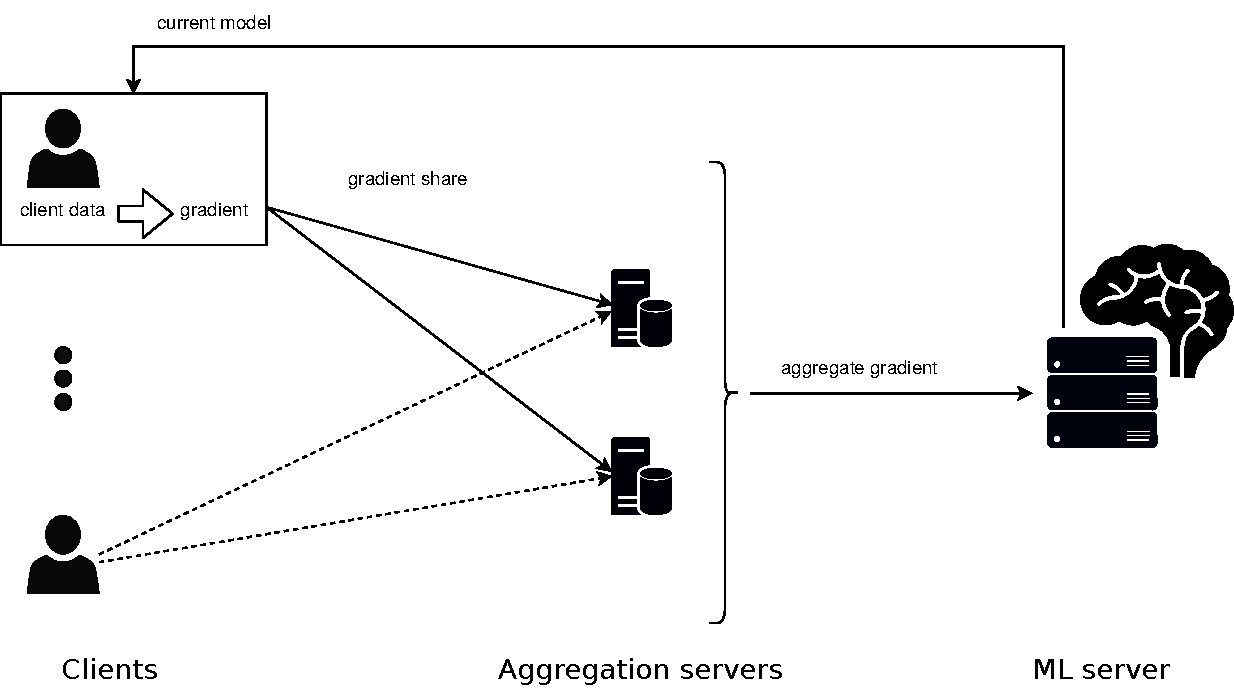
\includegraphics[width=\columnwidth]{assets/dpsa-overview-2-edit_no_explanations-2023-08-22.drawio.pdf}
  \caption{Test}
  \label{fig:architecture}
\end{figure}

The FL framework, i.e., flower, remains responsible for all functions of an FL
scheme, except for gradient aggregation. This includes broadcasting of the
current model, selecting clients for training, and applying the aggregated
gradients to the model.

The janus servers are responsible for making the aggregation of clients'
gradients secure and private. These aggregation servers do not need to be
managed by the same organization that is running the FL scheme, since they
merely provide a generic aggregation mechanism. They are intended to be long
running services which are responsible for processing aggregation jobs for
various applications concurrently. In fact, the threat model assumes that at
least one aggregation server is run by a separate organization, see section ?.

\subsection{Threat model}
The controller and the clients have different goals, and thus the threat model
has to be considered seperately for them. The parties running the aggregation
servers should be impartial to the learning process, but of course might deviate
from that behaviour. We consider the perspectives of the clients
and of the controller below.

\paragraph{Clients.} The clients are interested in participating in an FL-scheme
without their private information becoming known by other parties. There are two
ways this might happen:
\begin{enumerate}
\item The submitted gradient vector of a client (for a given training round) might
  become known to other parties. This would allow them to infer properties of
  the local training set.
\item Access to the trained model makes it possible to make inferences about the
  combined training set. Combination with other publicly available data can lead to
  leakage of individual clients' data.
\end{enumerate}
Our system guarantees the following: As long as at least one aggregation server
follows the protocol (i.e., is honest-but-curious), the client's data remains
private. Attack (1) is mitigated by the secure aggregation mechanism of DAP.
As long as the aggregation servers don't collude, they don't have access to
individual gradients. Attack (2) is mitigated by the fact that the sum of
gradient vectors is never revealed by itself, but only together with the noise added by
both aggregation servers. As long as at least one aggregation server adds
correctly configured noise, this makes the revealed value differentially
private. Differential privacy mitigates inference attacks (source).

In practice this means: clients can be sure that their data is safe as long as
they trust one of the aggregation servers to be honest in their execution of the
protocol. No trust in the controller is required.

\paragraph{Controller.} The controller is interested in training an ML model on
the data of the clients. Since it cannot inspect the individually submitted
gradients, this introduces the possibility of data poisoning attacks: malicious
clients can try to influence the learning process by submitting exaggerated
gradient vectors.

The DAP is designed to mitigate this sort of attack. Even though the aggregation
servers do not have access to individual plaintext gradients, they have a
protocol for verifying that each of the submitted reports is well-formed, i.e.,
has an L2-norm less than $1$. This means that while clients still can submit
``false'' data, they cannot gain unproportional leverage by doing so. Thus, data
poisoning attacks by a minority of clients are mitigated. The DAP can only
guarantee this as long as the aggregation servers do not collude with malicious
clients, as in that case it would be easy to craft submissions to fool the other
aggregation server into believing that reports are well-formed, even though they
are not.

In practice this means: the controller can be sure that it receives gradients
based on real data, as long as it trusts \textit{both} aggregation servers to
execute the protocol honestly, and a majority of clients is honest.

\subsection{Intended setup.}

This means that an FL-org can delegate the additionally required infrastructure
to a ``DAP as a service''-provider, and thus get good privacy guarantees for
their users without too much organizational overhead.

\subsection{Execution}

We describe how a single round of an FL-scheme is executed:
\begin{enumerate}[itemsep=0mm]
\item The controller selects available clients for this round and broadcasts its model to them.
\item The clients train their copy of the model on their local training data and
  compute the overall gradient vector.
\item They encode and split the gradient vector according to the prio protocol
  and submit each part to an aggregation server.
\item The aggregation servers aggregate reports from all clients, verify them,
  add noise for differential privacy and compute the sum of all gradient vectors.
\item The controller gets this gradient vector, applies it to its model, and
  begins the next round.
\end{enumerate}
It is important to note that each aggregation server receives only a ``share''
of every clients' gradient vector. It is impossible to reconstruct the original
vector from this share alone. All processing on the aggregation server, i.e.,
the verification, aggregation and noising happens in terms of its shares.
Only the subsequent combination of the resuls from both aggregation servers gives
us a plaintext value: the sum of all gradient vectors, together with noise. From
this value too it is sufficiently improbable to conclude properties of
individual clients' submissions. See section  for a more detailed analysis.



\subsection{Implementation}
 The protocol describes a distributed implementation of the usual differentially private gradient descent \cite{Abadi_2016}, with the differences being the integer encoding of the gradient vector to enable secret sharing according to the prio protocol \cite{prio}, the aggregation happening on a different machine than the training itself, and the use of discrete Gaussian noise on the integer encoding of the gradient aggregate.
\begin{algorithm}[h]
  \caption{Client procedure}\label{alg:client}

  \begin{algorithmic}[1]
  \Require Training dataset $X$, loss function $\mathcal L(\theta; x)$, number of rounds $N$, fixed-point encoding bit length $b$, set of aggregator server adresses $\texttt{S}$
  \Ensure Model $\theta$ trained on dataset $X$ for $N$ rounds

  \State $\textbf{round}_{(b,0)}(x) = \textbf{sign}(x) \cdot \textbf{floor}_b(|x|)$ \Comment{round to $b$ bits towards zero}
  \State $\pi(x) = 2^{b-1}\cdot (x + 1)$ \Comment{project fixed-point $x\in(-1,1)$ to an integer $\leq 2^b$}

  \For{$N$}\label{lst:line:loop}
  \State$\theta$ = retrieve current shared model from controller\label{lst:line:retrieve}
  \State$\textbf{g}$ = $\frac{1}{|X|} \sum_{x\in X} \nabla\mathcal L(\theta; x)$ \Comment{compute model gradient average}
\label{lst:line:grad}
  \State$\textbf{g}_{clip}$ = $\textbf{g}/\mathbf{max}\{1,||\textbf{g}||_{L_2}\}$ \Comment{clip $\textbf{g}$ to $L_2$ norm 1}\label{lst:line:clip}
  \State$\textbf{g}_{fixed}$ = \Call{\textbf{map}}{$\textbf{round}_{(b,0)}$,$\textbf{g}_{clip}$} \Comment{round to get $b$-bit fixed-point vector}
  \State$\textbf{g}_{int}$ = \Call{\textbf{map}}{$\pi$,$\textbf{g}_{fixed}$} \Comment{project to integer vector}
\label{lst:line:project}
  \State send one secret share of $\textbf{g}_{int}$ to each of the aggregation servers in \texttt S
  \EndFor
  \State$\theta$ = retrieve current shared model from controller
  \State\Return $\theta$
  \end{algorithmic}
\end{algorithm}


\begin{algorithm}[h]
  \caption{Aggregator server procedure}\label{alg:server}
  \begin{algorithmic}[1]
  \Require Set of client adresses $\texttt{C}$, set of aggregator server adresses $\texttt{S}$, privacy parameter $\rho$, fixed-point encoding bit length $b$
  \Ensure Aggregate gradient, noised to be $\rho$-zero-concentrated differentially private

  \State$\textbf{verify}_{\texttt{S}}(\textbf x)$ = perform prio protocol with the other aggregators in \texttt{S} to verify $\textbf x$ is a share of a fixed-point vector with $L_2$ norm $\leq 1$ with entries projected to the integers $\{0,...,2^b\}$ using $\pi$
  \State$\textbf{decrypt}_{\texttt{S}}(\textbf x)$ = perform prio protocol with the other aggregators in \texttt{S} to combine their aggregate shares with $\textbf x$ and obtain the aggregation result
  \State$\textbf{noise}(x) = x+n$ where $n$ is drawn from a discrete Gaussian distribution $\mathcal N_\mathbb{Z}\left(0,\frac{2^{2b}}{2\rho}\right)$
  \State$\pi'(y) = 2^{1-b} \cdot y - |\texttt{C}|$ \Comment{project integer $\leq 2^b\cdot|\texttt{C}|$ to float}
  \State\textbf{G} = 0
  \For{all clients $\texttt{c} \in \texttt{C}$}
       \State{\textbf{g} = retrieve gradient share from \texttt{c}}
	   \State$\textbf{verify}_\texttt{S}(\textbf{g})$ \label{lst:line:verify}
	   \State\textbf{G} = \textbf{G} + \textbf{g}
  \EndFor
  \State$\textbf{G}_{noised} = \textbf{map}(\textbf{noise}, \textbf{G})$  \Comment{add noise componentwise} \label{lst:line:noise}
  \State$\textbf{G}_{agg} = \textbf{decrypt}_{\texttt{S}}(\textbf{G}_{noised})$ \Comment{combine shares to aggregate}
  \State$\textbf{G}_{float} = \textbf{map}(\pi', \textbf{G}_{agg})$ \Comment{map to float vector}
  \State send $\textbf{G}_{float}$ to controller
  \end{algorithmic}
\end{algorithm}

\section{Privacy analysis}
We claim that executing Algorithms 1 and 2 with non-colluding aggregation servers, one of which honestly but curiously follows protocol, and an arbitrary number of potentially malicious clients, provides $(N \cdot \rho)$-zero-concentrated differential privacy for any clients' dataset. If both servers are honest, the protocol also protects against data poisoning attacks by malicious clients.

\paragraph{Privacy}
We perform the privacy analysis from the point of view of one client executing one iteration of the loop starting at line~\ref{lst:line:loop} of Algorithm~\ref{alg:client} faithfully. We show that:
\begin{enumerate}
\item The function mapping the clients' dataset to the gradient whose shares are transferred to the aggregation servers is $2^b$-sensitive.
\item No information about the gradient except its secret shares is revealed to any party prior to noising.
\item The noise added on the aggregation server provides $\rho$-zero-concentrated differential privacy for the aggregation result.
\end{enumerate}
It follows that the execution of Algorithm~\ref{alg:client} provides $(N\cdot\rho)$-zero-concentrated differential privacy by the composition property \cite[Lemma~1.8 on page 7]{DBLP:journals/corr/BunS16}.

\begin{enumerate}
\item We want to determine the sensitivity in the dataset $X$ of one iteration of the loop starting at line~\ref{lst:line:loop} of Algorithm~\ref{alg:client}. Assuming the current shared model $\theta$ retrieved in line~\ref{lst:line:retrieve} was computed in a way that provides differential privacy for $X$, its use will not affect the sensitvity. The clipping in line~\ref{lst:line:clip} ensures that 
\[\|\textbf{g}_{fixed}\|_2 = \|\overline{\textbf{round}}_{(b,0)}(\textbf{g}_{clip})\|_2\leq\|\textbf{g}_{clip}\|_2\leq 1.\]
Denote by $\textbf{g}'$ the values of the variables in the algorithm obtained by replacing any one entry in $X$ by a different entry, and by $\overline\pi$ the component-wise application of the function $\pi$. We have
\begin{align*}
\|\textbf g_{int} - \textbf g_{int}'\|_2 &= \|\overline\pi(\textbf g_{fixed}) - \overline \pi(\textbf g_{fixed}')\|_2 \\
&\leq 2^{b-1} \cdot \| \textbf g_{fixed}- \textbf g_{fixed}'\|_2\\
&\leq 2^{b-1} \cdot (\| \textbf g_{fixed}\|_2 + \|\textbf g_{fixed}'\|_2)\\
&\leq 2^b
\end{align*}
One iteration of the computation inside the loop (lines~\ref{lst:line:retrieve} to \ref{lst:line:project}) therefore is $2^b$-sensitive in $X$.

\item Prio secret sharing amounts to the client splitting their secret into summands, and recovering the aggregated shares amounts to summing the sums of secret shares \cite[Scheme on page 3]{prio}. Doing so does not affect the sensitivity of $\textbf{g}_{int}$, as the result of the computation is equal to the result obtained by summing all clients' gradients without secret sharing. Share transfer happens over an encrypted channel \cite[Step 1 of Scheme on page 3]{prio}, combining the shares happens after adding noise on the server in line~\ref{lst:line:noise}. Therefore if at least one of the servers is honest and they don't collude, the only things visible to anyone evesdropping or participating are single secret shares of the gradient and the noised aggregate.

\item Noise is added prior to combining the aggregate shares to avoid disclosing the non-noised aggregate to a server. Since combining them simply means computing their sum \cite[Step 3 of Scheme on page 3]{prio}, the value of $\textbf{G}_{agg}$ does not depend on whether the noise is added before or after combining the shares. We can hence view the function mapping one clients' data set $X$ to the non-noised gradient aggregate as a $2^b$-sensitive function over the integers, so adding noise drawn from $\mathcal N_\mathbb{Z}\left(0,\frac{2^{2b}}{2\rho}\right)$ will provide $\rho$-zero-concentrated differential privacy due to~\cite[Theorem 14 on page 15, with all $\sigma_j=\frac{2^{2b}}{2\rho}$]{DBLP:journals/corr/abs-2004-00010}. Mapping the integer encoding of the aggregate back to a float vector and using it in further training will not affect privacy due to post-processing invariance. Note that each server adds the entire amount of noise required to obtain the guarantee, so if at least one of them is honest the guarantee holds. This comes at the cost of adding the entire noise on each server, resulting in worse utility.
\end{enumerate}

\paragraph{Robustness}
In line~\ref{lst:line:verify} of Algorithm~\ref{alg:server}, the servers perform a secret-shared non-interactive proof protocol \cite[Section 4]{prio} together to verify that the client-side clipping was performed properly. This ensures the sensitivity is as described above, even for gradients submitted by malicious clients, and hence protects from clients attempting data poisoning, i.e. influencing the computation result in a way that benefits them. The verification part of the protocol requires all servers to act honestly, so our system offers this protection only under a weaker threat model. The above proof of privacy still holds for all clients that execute the protocol truthfully.

\section{Evaluation}

\subsection{Utility analysis}
We want to know how much noise our algorithm adds compared to the standard gradient descent with differential privacy obtained by sampling from the regular normal distribution~\cite{Abadi_2016}. There, each iteration of gradient aggregation adds noise drawn from $\mathcal N\left(0,\frac{(2C)^2}{2\rho}\right)$ for gradients clipped to norm $C$ ($C=1$, in our case) and our notion of $\rho$-zero-concentrated differential privacy.

Consider rounding both gradient entries and noise to obtain $b$-bit fixed point numbers with one integer bit. Rounding a gradient introduces an error
$$|\textbf{round}_{0,b)}(x) - x|\leq\frac{1}{2^{b-1}}$$
to each of the clients' gradient entries in each aggregation step. This should be negligible given that the noise added to each aggregate entry is sampled from a normal distribution with standard deviation of $\sqrt{\frac{2}{\rho}}$, meaning that even for large values of $\rho$, say $\rho = 2^6$, and small values of $b$, say $b=16$, still $99.88\%$ of the noise samples will be an order of magnitude larger than that error.

Next consider applying the projection $\pi$ to both gradients and noise before applying the noise, and reversing the projection afterwards. This does not alter the magnitude of the noise in the end result, and is equivalent to sampling instead from a scaled rounded Gaussian distribution $\mathcal N_{round}\left(0,\frac{2^{2b}}{2\rho}\right)$.

Next consider using the discrete Gaussian instead. \cite[Corollary 17]{DBLP:journals/corr/abs-2004-00010} shows that utility is strictly better by a small amount.

Last, consider that our protocol simply is a modification of the regular gradient descent algorithm with differential privacy as described in this section, but the aggreagtion and addition of noise is distributed among multiple servers $\texttt{S}$. As described in our threat model, in order to require trust in only one of those servers, each server has to add the entire amount of noise, so noise magnitude worsens by a multiple of $|\texttt{S}|$. The sum of discrete Gaussian variables is distributed closely Gaussian~\cite[Theorem 11]{Kairouz2021TheDD}, so utility of our algorithm with $\rho$-ZCdp is approximately that of the regular gradient descent with $|\texttt{S}|\cdot\rho$-ZCdp. If all aggregators are trustworthy, the protocol can be adapted so each only adds a fraction of the total noise to improve utility while maintaining the privacy bound.


\subsection{Communication complexity}
The communication costs of transmitting the clients' gradients in a
differentially private way, compared to transmitting plaintext data is an
important metric for evaluating aggregation protocols for FL. Since gradients
are typically large (e.g. [TODO: insert size here]), their transmission accounts
for most of the time complexity of the whole learning procedure.

In the prio protocol, the message size is mostly determined by the size of the
encoded gradient together with the size of the encoded proof of its
well-formedness. Such a message has to be sent two times: one to the leader and
one to the helper. Other messages sent as part of the prio protocol are negligible.

In our current implementation of \texttt{dpsa4fl} we use a naive encoding of
gradient entries as field elements. This results in a rather large blow-up of
message size. Improvements to our encoding are incoming, and as such we don't
desribe our encoding in detail. It should suffice to say that currently, a
single 16-bit fixed point number is encoded by 16 128-bit field elements, which
means that our messages are at least 128 times the size of plaintext gradients.
There are both trivial and more complex methods to improve on this: the field
size of 128-bit can be reduced to 64-bit while still supporting gradients with
up to $2^{34} \approx 17 \cdot 10^9$ entries. Furthermore, the encoding can be
compactified, such as not to require a seperate field element for each
transmitted bit. Since this will increase the size of the correctness proof,
a balance which optimizes message size has to be found.


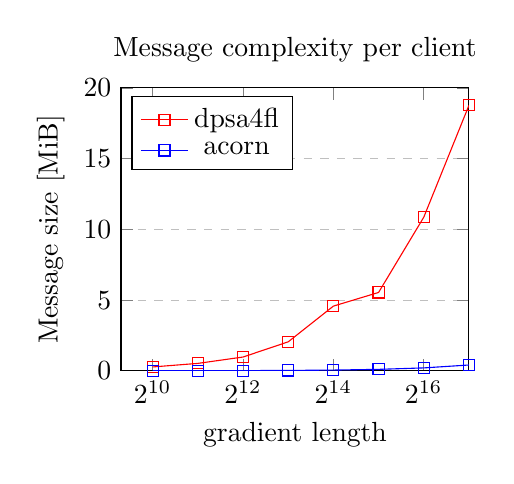
\begin{tikzpicture}
  \begin{axis}[
    title={Message complexity per client},
    xlabel={gradient length},
    ylabel={Message size [MiB]},
    xmode=log,
    log basis x=2,
    xlabel=gradient length,
    ymode=normal,
    % ymode=log,
    % log ticks with fixed point,
    xmin=0, xmax=2^17,
    ymin=0, ymax=20,
    % xtick={0,20,40,60,80,100},
    % ytick={0,20,40,60,80,100,120},
    legend pos=north west,
    ymajorgrids=true,
    grid style=dashed,
    ]

    \addplot[
    color=red,
    mark=square,
    ]
    coordinates {
      (2^10,0.2738359375)(2^11,0.525400390625)(2^12,0.97528125)(2^13,2.049)(2^14,4.574)(2^15,5.539)(2^16,10.855)(2^17,18.761)
    };
    \addlegendentry{dpsa4fl}

    \addplot[
    color=blue,
    mark=square,
    ]
    coordinates {
      (2^10,0.0044921875)(2^11,0.00771484375)(2^12,0.0142578125)(2^13,0.02705078125)(2^14,0.052734375)(2^15,0.10400390625)(2^16,0.2064453125)(2^17,0.411328125)
    };
    \addlegendentry{acorn}
  \end{axis}
\end{tikzpicture}




\section{Conclusion}

\bibliographystyle{plain}
\bibliography{refs}

\end{document}

